\documentclass{article}

\usepackage[utf8]{inputenc}
\usepackage[T1]{fontenc}
\usepackage{lmodern}
\usepackage{amsmath}
\usepackage{amssymb}
\usepackage{amsthm}
\usepackage{mathtools}
\usepackage{empheq}
\usepackage{parskip}
\usepackage{hyperref}
\usepackage{cleveref}
\usepackage{graphicx}
\usepackage{booktabs}
\usepackage{float}

\usepackage[margin=0.75in]{geometry}

\usepackage{pgfplots}
\pgfplotsset{compat=1.18}

\title{Hysteresis Lab Report}
\author{London Wallace | 23071503}
\date{}

\setlength{\parindent}{0pt}
\setlength{\parskip}{1em plus 0.1em minus 0.1em}

\begin{document}

\maketitle{}

\begin{flushleft}
	\textbf{Due Date:} May 2, 2026, 11:59 PM
\end{flushleft}

\section{Introduction}

On Friday, May 1, 2026 an experiment was conducted with the goal of observing and measuring the hysteresis loops,
magnetisation curves, and Curie temperatures of various unknown ferrite materials.

Ferromagnetism is a property of some materials that results in significant magnetic permeability and
coercivity \cite{ferromagnetism-wiki}, which is the
amount of induced magnetism in a material in response to an external magnetic field \cite{permeability-wiki} and its ability
to resist becoming demagnetised \cite{coercivity-wiki}, respectively, allowing it to form a permanent magnet. It is the phenomenon most
associated with \emph{magnetism} in the vernacular. The Curie temperature of a ferromagnetic material is the point at which the thermal
interactions of the atoms overwhelm the materials coercivity, resulting in it losing its magnetic properties \cite{lab-manual}.

A hysteresis loop is a plot of external magnetic field (H) vs. magnetisation (B) \cite{hysteresis}. (\cref{fig:example-hysteresis})
\begin{figure}[htbp]
	\centering
	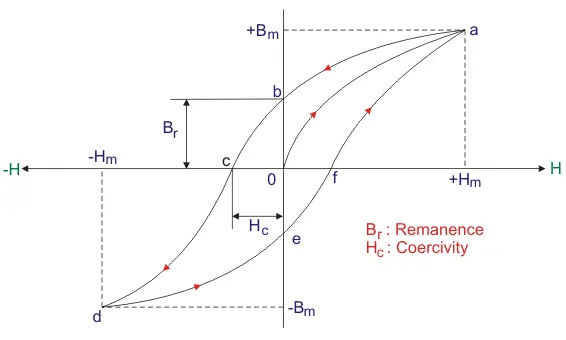
\includegraphics[width=0.8\textwidth]{hysterisis.png}
	\caption{Example Hysteresis Curve.}
	\label{fig:example-hysteresis}
\end{figure}

The magnetisation associated with 0 external magnetic field is called remanence (b). This is the magnetisation of a permanent
magnet. The point at which no more magnetisation can be induced regardless of the strength of the external field is called
saturation (a). The coercivity, or coercive force, is $|c|$, which is the opposite field strength required to demagnetise the ferromagnet.

The magnetisation curve is the path traced by the saturation point (a) when the external magnetic field strength is increased.
It is represented by the line from the origin to $a$ in the example. \cite{hysteresis} \cite{lab-manual}

\subsection{Equipment List}
\begin{enumerate}
	\item Digital Oscilloscope
	\item LEAI-71 (Signal Generator (a) and Hysteresis Loop Measurement Circuit (b)) (\cref{fig:blank-leai-71})
	\item Assorted cables
\end{enumerate}
\begin{figure}[htbp]
	\centering
	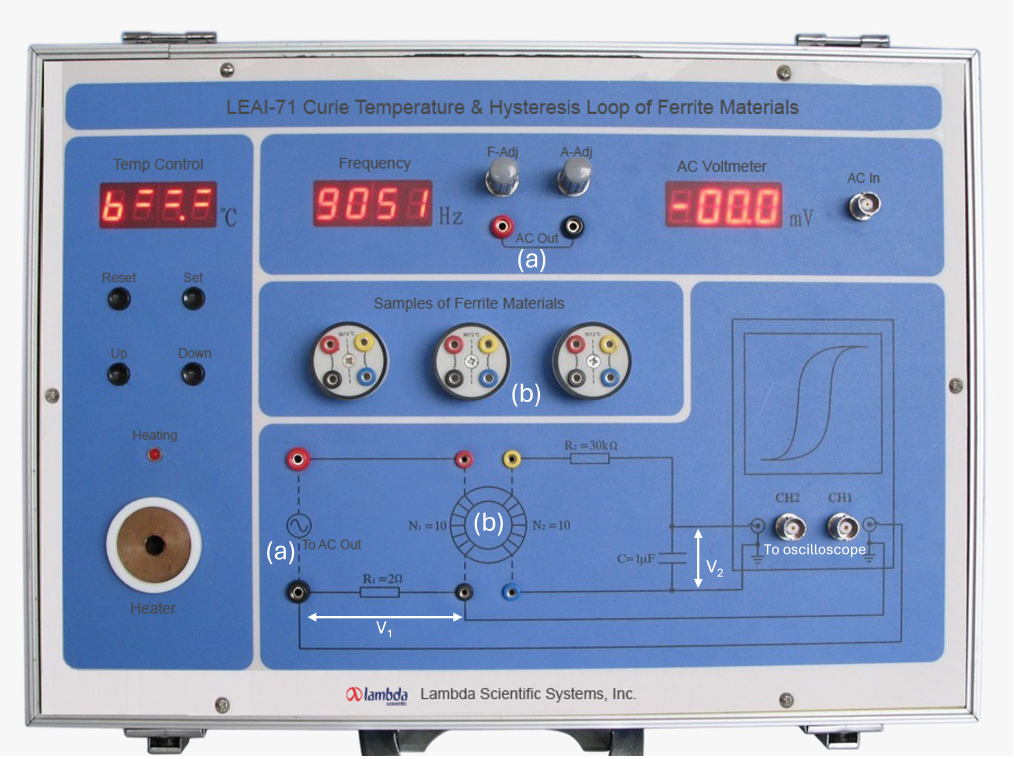
\includegraphics[width=0.8\textwidth]{leai-71.png}
	\caption{LEAI-71 before any wiring or connections. \cite{lab-manual}}
	\label{fig:blank-leai-71}
\end{figure}

\section{Method and Results}
\subsection{Method for Hysteresis Loop and Magnetisation Curve Measurement}
\begin{enumerate}
	\item The LEAI-71 was wired according to Figure 10 in the Lab Manual. The oscilloscope was set up according to the steps laid out in
	      the lab manual. The LEAI-71 was switched on to warm up for 10 minutes.
	\item The sample was connected to the LEAI-71 per Figure 10.
	\item The frequency was set to 7514 Hz (lowest possible) and the magnetising current set to 0.
	\item The channel 1 and channel 2 grid spacings were set to 20mV and 10mV respectively. Channel 1 was adjusted -5.25mV and channel 2
	      -300mV to place the data signal at the origin.
	\item Magnetising current was increased to maximum and grid spacing adjusted to 60mV/12.5mV to fit the entire curve to the screen.
	\item The sample was demagnetised by slowly reducing the magnetising current.
	\item The magnetising current was slowly increased until saturation.
	\item Oscilloscope cursors were used to measure apparent $H_m, B_m, H_c, B_r$
	\item The sample was demagnetised again.
	\item The magnetising current was slowly increased until saturation, with readings of apparent $H_m, B_m$ every 5mV to measure
	      magnetising curve.
	\item Sample was demagnetised and swapped. Steps 2-11 were repeated for Samples A and B.
\end{enumerate}

\subsection{Hysteresis Loop Results}
\begin{table}[H]
	\begin{center}



		\begin{tabular}{ccccc}
			\toprule
			Sample & $H_m$ (mV) & $B_m$ (mV) & $H_c$ (mV) & $B_r$ (mV) \\
			\midrule
			A      & 318.75     & 45.775     & -54.000    & 27.175     \\
			B      & 369.90     & 47.025     & -29.400    & 24.675     \\
			\bottomrule
		\end{tabular}

	\end{center}
	\caption{Apparent (measured) hysteresis loop results for Sample A and B.}
\end{table}

These apparent values were converted by the given equations
\begin{align}
	H & = \dfrac{N_1 \cdot V_1}{l \cdot R_1}         \\
	B & = \dfrac{R_2 \cdot C \cdot V_2}{N_2 \cdot S}
\end{align}
Where $l=13.8$mm, $S=6.4\text{mm}^2$, $C=1\mu F$, $R_1=2\Omega$, $R_2=300\Omega$, $N_1=N_2=10$ and $V_1$ is the $x$-component
measured from the oscilloscope ($H_m, H_c$) and $V_2$ is the $y$-component ($B_m, B_r$).

These carry dimensions
\begin{align*}
	H & = \dfrac{\text{mV}}{\text{mm} \cdot \Omega} = \dfrac{\text{Amperes}}{\text{Meter}}                                      \\
	B & = \dfrac{\Omega \cdot \mu F \cdot \text{mV}}{\text{mm}^2} = \text{m}\dfrac{\text{Webber}}{\text{Meter}^2}=\text{mTesla}
\end{align*}

Giving the converted results
\begin{table}[H]
	\begin{center}
		\begin{tabular}{ccccc}
			\toprule
			Sample & $H_{\text{saturation}}$ (Am$^{-1}$) & $B_{\text{saturation}}$ (mT) & $H_{\text{coercivity}}$ (Am$^{-1}$) & $B_{\text{remanance}}$ (mT) \\
			\midrule
			A      & 115.49                              & 214.57                       & -19.565                             & 127.38                      \\
			B      & 134.02                              & 220.43                       & -10.652                             & 115.66                      \\
			\bottomrule
		\end{tabular}
	\end{center}
	\caption{Converted hysteresis loops results (via (1) and (2)) for Samples A and B.}
\end{table}
The raw data was saved from the oscilloscope and parsed with a python script available at
\url{https://codeberg.org/londonwallace/bmath/src/branch/main/PHYS2001/Hysteresis/convert_csv.py}
and plotted. The $B_m, H_m, B_r,$ and $H_c$ points were marked using the measured value in the table above and were not re-derived
from the raw CSV data.
\begin{figure}[p]
	\vfill
	\begin{tikzpicture}
		\begin{axis}[
				xlabel={H (V)},
				ylabel={B (V)},
				grid=major,
				width=\textwidth,
				height=10cm,
				axis lines=middle,
				axis line style={thick, black},
				xtick={-0.4,-0.3,-0.2,-0.1,0,0.1,0.2,0.3,0.4},
				xticklabel style={font=\footnotesize},
				yticklabel style={font=\footnotesize},
				scaled y ticks=false,
				scaled x ticks=false,
				enlarge x limits=0.1,
				enlarge y limits=0.1,
			]
			\addplot [
				color=black,
				mark=*,
				mark size=1pt,
				thick
			] table [
					x index=1,
					y index=2,
					col sep=comma
				] {scope_39.output.csv};

			\node[black, anchor=east] at (axis cs:0, .045775) {$B_m$};
			\draw[black, thick] (axis cs:0.31875, 0.045775) -- (axis cs:0, 0.045775);
			\draw[black, thick] (axis cs:0.31875, 0.045775) -- (axis cs:0.31875, 0);
			\node[black, anchor=north] at (axis cs:0.31875, 0) {$H_m$};
			\draw[red, thick] (axis cs:-0.054, 0) -- (axis cs:0, 0);
			\node[red, anchor=north west] at (axis cs:-0.054, 0) {$H_c$};
			\draw[red, thick] (axis cs:0, 0.027175) -- (axis cs:0, 0);
			\node[red, anchor=east] at (axis cs:0, 0.027175) {$B_r$};

		\end{axis}
	\end{tikzpicture}
	\caption{Sample A Hysteresis Plot.}
\end{figure}
\begin{figure}[p]
	\vfill
	\begin{tikzpicture}
		\begin{axis}[
				xlabel={H (V)},
				ylabel={B (V)},
				grid=major,
				width=\textwidth,
				height=10cm,
				axis lines=middle,
				axis line style={thick, black},
				xtick={-0.4,-0.3,-0.2,-0.1,0,0.1,0.2,0.3,0.4},
				xticklabel style={font=\footnotesize},
				yticklabel style={font=\footnotesize},
				scaled y ticks=false,
				scaled x ticks=false,
				enlarge x limits=0.1,
				enlarge y limits=0.1,
			]
			\addplot [
				color=black,
				mark=*,
				mark size=1pt,
				thick
			] table [
					x index=1,
					y index=2,
					col sep=comma
				] {scope_41.output.csv};

			\node[black, anchor=east] at (axis cs:0, .047025) {$B_m$};
			\draw[black, thick] (axis cs:0.36990, 0.047025) -- (axis cs:0, 0.047025);
			\draw[black, thick] (axis cs:0.36990, 0.047025) -- (axis cs:0.36990, 0);
			\node[black, anchor=north] at (axis cs:0.36990, 0) {$H_m$};
			\draw[red, thick] (axis cs:-0.0294, 0) -- (axis cs:0, 0);
			\node[red, anchor=north west] at (axis cs:-0.0294, 0) {$H_c$};
			\draw[red, thick] (axis cs:0, 0.024675) -- (axis cs:0, 0);
			\node[red, anchor=east] at (axis cs:0, 0.024675) {$B_r$};

		\end{axis}
	\end{tikzpicture}
	\caption{Sample B Hysteresis Plot.}
\end{figure}
\vfill
\newpage
\subsection{Magnetising Curve Results}
\begin{table}[h]
	\centering
	\begin{minipage}{0.48\textwidth}
		\centering
		\textbf{Sample A}\\[0.5em]
		\begin{tabular}{cc}
			\toprule
			$H_m$ (mV) & $B_m$ (mV) \\
			\midrule
			5          & 28         \\
			10         & 48         \\
			15         & 63         \\
			20         & 75         \\
			25         & 87         \\
			30         & 96         \\
			35         & 106        \\
			40         & 117        \\
			45         & 129        \\
			50         & 140        \\
			55         & 154        \\
			60         & 171        \\
			65         & 196        \\
			70         & 230        \\
			75         & 285        \\
			80         & 370        \\
			85         & 504        \\
			90         & 745        \\
			\bottomrule
		\end{tabular}
	\end{minipage}%
	\hfill
	\begin{minipage}{0.48\textwidth}
		\centering
		\textbf{Sample B}\\[0.5em]
		\begin{tabular}{cc}
			\toprule
			$H_m$ (mV) & $B_m$ (mV) \\
			\midrule
			5          & 22         \\
			10         & 34         \\
			20         & 50         \\
			25         & 57         \\
			30         & 64         \\
			35         & 71         \\
			50         & 79         \\
			45         & 86         \\
			50         & 94         \\
			55         & 104        \\
			60         & 118        \\
			65         & 135        \\
			70         & 156        \\
			75         & 194        \\
			80         & 265        \\
			85         & 390        \\
			90         & 654        \\
			91         & 766        \\
			\bottomrule
		\end{tabular}
	\end{minipage}
	\caption{Apparent (measured) magnetising curve results for Sample A (left) and Sample B (right).}
\end{table}
Equations (1) and (2) were used, as well as
\begin{equation}
	\mu = \dfrac{B}{H}
\end{equation}
To convert these apparent values to their respective H, B, and $\mu$. Permeability $\mu$ carries the dimensions
\begin{equation*}
	\dfrac{\text{mT}}{\dfrac{\text{Amperes}}{\text{Meter}}} = \dfrac{\text{mT}\cdot\text{m}}{\text{A}}=\dfrac{\text{mH}}{\text{m}}
\end{equation*}
Results of this conversion are found in \cref{4}. These converted values of magnetisation and permeability were plotted against
external field strength for Sample A (\cref{5}) and Sample B (\cref{6}). Permeability was scaled by a factor of 10 to better
illustrate the relationship between permeability and magnetisation on the available grid spacing.
\begin{table}[h]

	\centering
	\begin{minipage}{0.48\textwidth}
		\centering
		\textbf{Sample A}\\[0.5em]
		\begin{tabular}{ccc}
			\toprule
			$H_m$ (Am$^{-1}$) & $B_m$ (mT) & $\mu$ (mH$\cdot$m$^{-1}$) \\
			\midrule
			1.81              & 28         & 15.46                     \\
			3.62              & 48         & 13.25                     \\
			5.43              & 63         & 11.60                     \\
			7.24              & 75         & 10.35                     \\
			9.05              & 87         & 9.61                      \\
			10.86             & 96         & 8.83                      \\
			12.67             & 106        & 8.36                      \\
			14.48             & 117        & 8.08                      \\
			16.29             & 129        & 7.91                      \\
			18.1              & 140        & 7.73                      \\
			19.91             & 154        & 7.73                      \\
			21.72             & 171        & 7.87                      \\
			23.52             & 196        & 8.32                      \\
			25.34             & 230        & 9.07                      \\
			27.15             & 285        & 10.49                     \\
			28.96             & 370        & 12.77                     \\
			30.77             & 504        & 16.37                     \\
			32.58             & 745        & 22.86                     \\
			\bottomrule
		\end{tabular}
	\end{minipage}%
	\hfill
	\begin{minipage}{0.48\textwidth}
		\centering
		\textbf{Sample B}\\[0.5em]
		\begin{tabular}{ccc}
			\toprule
			$H_m$ (Am$^{-1}$) & $B_m$ (mT) & $\mu$ (mH$\cdot$m$^{-1}$) \\
			\midrule
			1.81              & 22         & 12.15                     \\
			3.62              & 34         & 9.39                      \\
			7.24              & 50         & 6.90                      \\
			9.05              & 57         & 6.29                      \\
			10.86             & 64         & 5.89                      \\
			12.67             & 71         & 5.60                      \\
			14.48             & 79         & 5.45                      \\
			16.29             & 86         & 5.27                      \\
			18.1              & 94         & 5.19                      \\
			19.91             & 104        & 5.22                      \\
			21.72             & 118        & 5.43                      \\
			23.52             & 135        & 5.737                     \\
			25.34             & 156        & 6.15                      \\
			27.15             & 194        & 7.14                      \\
			28.96             & 265        & 9.15                      \\
			30.77             & 390        & 12.67                     \\
			32.58             & 654        & 20.07                     \\
			32.94             & 766        & 23.25                     \\
			\bottomrule
		\end{tabular}
	\end{minipage}
	\caption{Converted magnetic field strength (H) and magnetisation (B), and derived permeability ($\mu$)
		for Sample A (left) and Sample B (right).}
	\label{4}
\end{table}
\begin{figure}[H]
	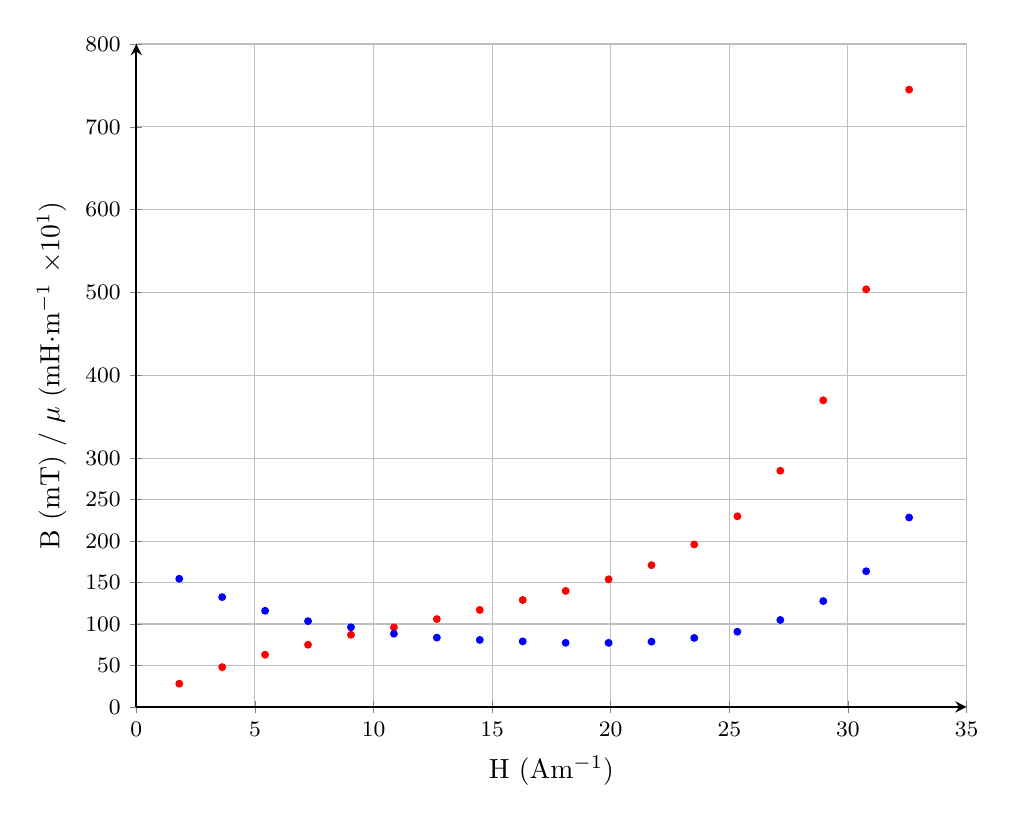
\begin{tikzpicture}
		\begin{axis}[
				xlabel={H (Am$^{-1}$)},
				ylabel={B (mT) / $\mu$ (mH$\cdot$m$^{-1}$} $\times 10^1$),
				grid=major,
				width=\textwidth,
				height=10cm,
				axis lines=left,
				axis line style={thick, black},
				xtick={0,5,10,15,20,25,30,35},
				ytick={0,50,100,150,200,250,300,400,500,600,700,800},
				xticklabel style={font=\footnotesize},
				yticklabel style={font=\footnotesize},
				scaled y ticks=false,
				scaled x ticks=false,
				xmax=35,
				ymax=800,
				xmin=0,
				ymin=0,
			]
			\addplot [only marks, mark=*, mark size=1pt, color=red, thick] coordinates {
					(1.81,28)
					(3.62,48)
					(5.43,63)
					(7.24,75)
					(9.05,87)
					(10.86,96)
					(12.67,106)
					(14.48,117)
					(16.29,129)
					(18.1,140)
					(19.91,154)
					(21.72,171)
					(23.52,196)
					(25.34,230)
					(27.15,285)
					(28.96,370)
					(30.77,504)
					(32.58,745)
				};
			\addplot [only marks, mark=*, mark size=1pt, color=blue, thick] coordinates {
					(1.81,154.6)
					(3.62,132.5)
					(5.43,116)
					(7.24,103.5)
					(9.05,96.1)
					(10.86,88.3)
					(12.67,83.6)
					(14.48,80.8)
					(16.29,79.1)
					(18.1,77.3)
					(19.91,77.3)
					(21.72,78.7)
					(23.52,83.2)
					(25.34,90.7)
					(27.15,104.9)
					(28.96,127.7)
					(30.77,163.7)
					(32.58,228.6)
				};
		\end{axis}
	\end{tikzpicture}
	\caption{Sample A's relationship between magnetisation B (red) and permeability
		$\mu$ (blue) with external field strength H. Permeability has been scaled by a factor of 10.}
	\label{5}
\end{figure}
\begin{figure}[H]
	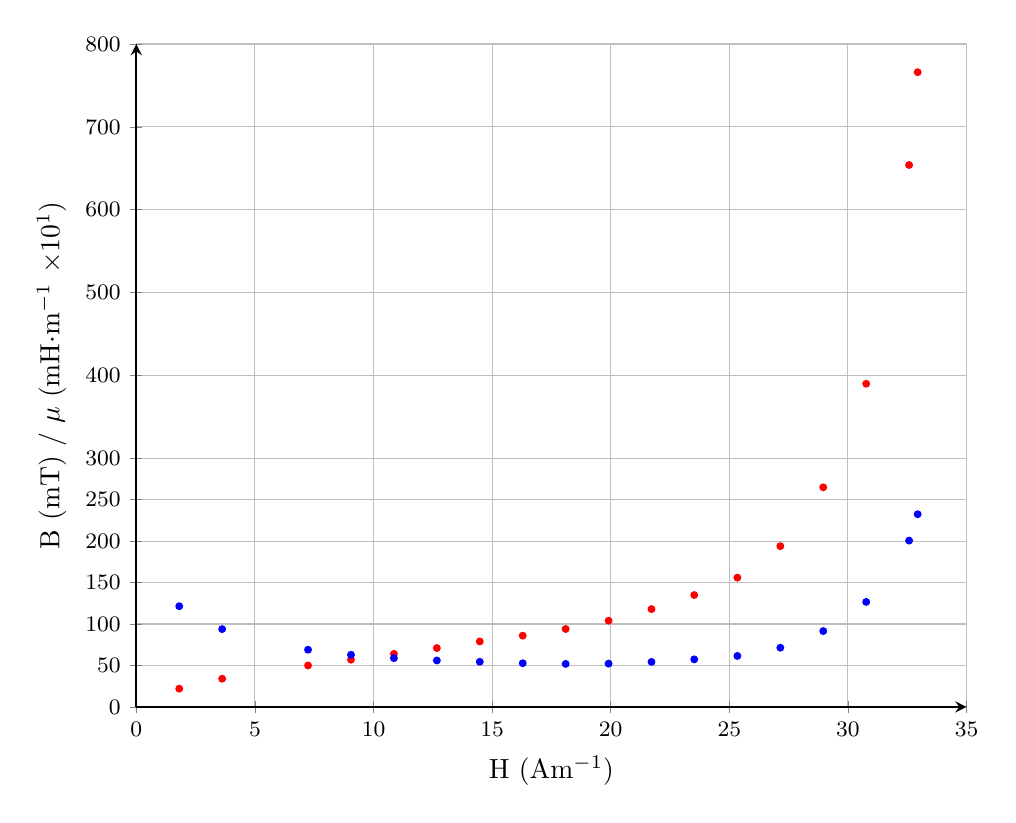
\begin{tikzpicture}
		\begin{axis}[
				xlabel={H (Am$^{-1}$)},
				ylabel={B (mT) / $\mu$ (mH$\cdot$m$^{-1}$} $\times 10^1$),
				grid=major,
				width=\textwidth,
				height=10cm,
				axis lines=left,
				axis line style={thick, black},
				xtick={0,5,10,15,20,25,30,35},
				ytick={0,50,100,150,200,250,300,400,500,600,700,800},
				xticklabel style={font=\footnotesize},
				yticklabel style={font=\footnotesize},
				scaled y ticks=false,
				scaled x ticks=false,
				xmax=35,
				ymax=800,
				xmin=0,
				ymin=0,
			]
			\addplot [only marks, mark=*, mark size=1pt, color=red, thick] coordinates {
					(1.81,22)
					(3.62,34)

					(7.24,50)
					(9.05,57)
					(10.86,64)
					(12.67,71)
					(14.48,79)
					(16.29,86)
					(18.1,94)
					(19.91,104)
					(21.72,118)
					(23.52,135)
					(25.34,156)
					(27.15,194)
					(28.96,265)
					(30.77,390)
					(32.58,654)
					(32.94,766)
				};
			\addplot [only marks, mark=*, mark size=1pt, color=blue, thick] coordinates {
					(1.81,121.5)
					(3.62,93.9)

					(7.24,69)
					(9.05,62.9)
					(10.86,58.9)
					(12.67,56)
					(14.48,54.5)
					(16.29,52.7)
					(18.1,51.9)
					(19.91,52.2)
					(21.72,54.3)
					(23.52,57.37)
					(25.34,61.5)
					(27.15,71.4)
					(28.96,91.5)
					(30.77,126.7)
					(32.58,200.7)
					(32.94,232.5)
				};
		\end{axis}
	\end{tikzpicture}
	\caption{Sample B's relationship between magnetisation B (red) and permeability
		$\mu$ (blue) with external field strength H. Permeability has been scaled by a factor of 10.}
	\label{6}
\end{figure}
\subsection{Method for Curie Temperature Measurement}
\begin{enumerate}
	\item Sample A was connected to the LEAI-71 according to Figure 10 of the lab manual.
\end{enumerate}

\section{Discussion}

Error analysis

Discussion of the final results.

\bibliographystyle{unsrt}
\bibliography{refs}

\end{document}
